\documentclass[tikz,border=12pt]{standalone}
\usepackage[utf8]{inputenc}\usepackage[T1]{fontenc}\usepackage{tikz}
\usetikzlibrary{arrows.meta,positioning,shadows.blur,shapes.geometric}
\definecolor{greenFill}{HTML}{E8F5E9}\definecolor{greenStroke}{HTML}{43A047}
\definecolor{coreFill}{HTML}{E1F5FE}\definecolor{coreStroke}{HTML}{0277BD}
\definecolor{optFill}{HTML}{FCE4EC}\definecolor{optStroke}{HTML}{D81B60}
\definecolor{memFill}{HTML}{FFF3E0}\definecolor{memStroke}{HTML}{EF8C00}
\begin{document}
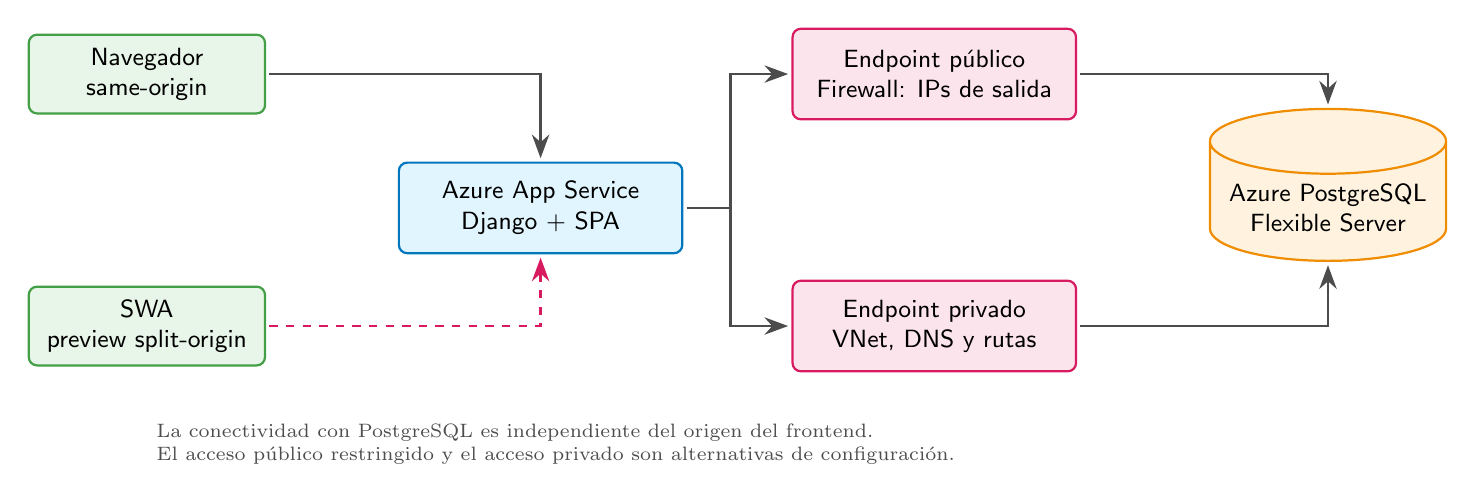
\begin{tikzpicture}[
  font=\sffamily\small,>={Stealth[length=3mm,width=2.2mm]},
  client/.style={rectangle,rounded corners=3pt,draw=greenStroke,thick,fill=greenFill,minimum width=3.0cm,minimum height=1.0cm,align=center},
  app/.style={rectangle,rounded corners=3pt,draw=coreStroke,thick,fill=coreFill,minimum width=3.6cm,minimum height=1.15cm,align=center},
  net/.style={rectangle,rounded corners=3pt,draw=optStroke,thick,fill=optFill,minimum width=3.6cm,minimum height=1.15cm,align=center},
  db/.style={cylinder,draw=memStroke,thick,aspect=0.3,shape border rotate=90,fill=memFill,minimum width=3.0cm,minimum height=1.5cm,align=center},
  edge/.style={->,line width=.9pt,draw=black!70,shorten >=1.2pt,shorten <=1.2pt}, optional/.style={->,line width=.9pt,dashed,draw=optStroke,shorten >=1.2pt,shorten <=1.2pt}
]
% The two incoming web paths reach the same application; database networking is shown separately.
\node[client] (same) at (0,1.7) {Navegador\\same-origin};
\node[client] (swa) at (0,-1.5) {SWA\\preview split-origin};
\node[app] (appservice) at (5,0) {Azure App Service\\Django + SPA};
\node[net] (public) at (10,1.7) {Endpoint público\\Firewall: IPs de salida};
\node[net] (vnet) at (10,-1.5) {Endpoint privado\\VNet, DNS y rutas};
\node[db] (postgres) at (15,0) {Azure PostgreSQL\\Flexible Server};
\draw[edge] (same.east) -| (appservice.north);
\draw[optional] (swa.east) -| (appservice.south);
\draw[edge] (appservice.east) -- ++(.6,0) |- (public.west);
\draw[edge] (appservice.east) -- ++(.6,0) |- (vnet.west);
\draw[edge] (public.east) -| (postgres.north);
\draw[edge] (vnet.east) -| (postgres.south);
\node[font=\scriptsize,text=black!70,align=left,anchor=west] at (0,-3.0)
 {La conectividad con PostgreSQL es independiente del origen del frontend.\\
  El acceso público restringido y el acceso privado son alternativas de configuración.};
\end{tikzpicture}
\end{document}
